% -------------------------------------------------------------------------------------- %

\documentclass[letterpaper,10pt]{article}



\pagestyle{empty}

\usepackage[table]{xcolor}
\usepackage{color, colortbl}
\usepackage{tabularx}
\usepackage{amssymb}
\usepackage{enumerate}

\definecolor{LightGray}{gray}{0.9}

\usepackage{amsmath}
\usepackage{amscd}
\usepackage{url}

\usepackage{graphicx}


\title{Installing AIMBAT}
\author{Seismo Group}
\date{\today}

\begin{document}
\maketitle

% -------------------------------------------------------------------------------------- %

\section{Getting your Operating System}

Go to \verb"System Preferences" as in~\ref{fig:system_preferences}, and click on \verb"Startup Disk". It should show your operation system version.

\begin{figure}[h!]
  \centering
  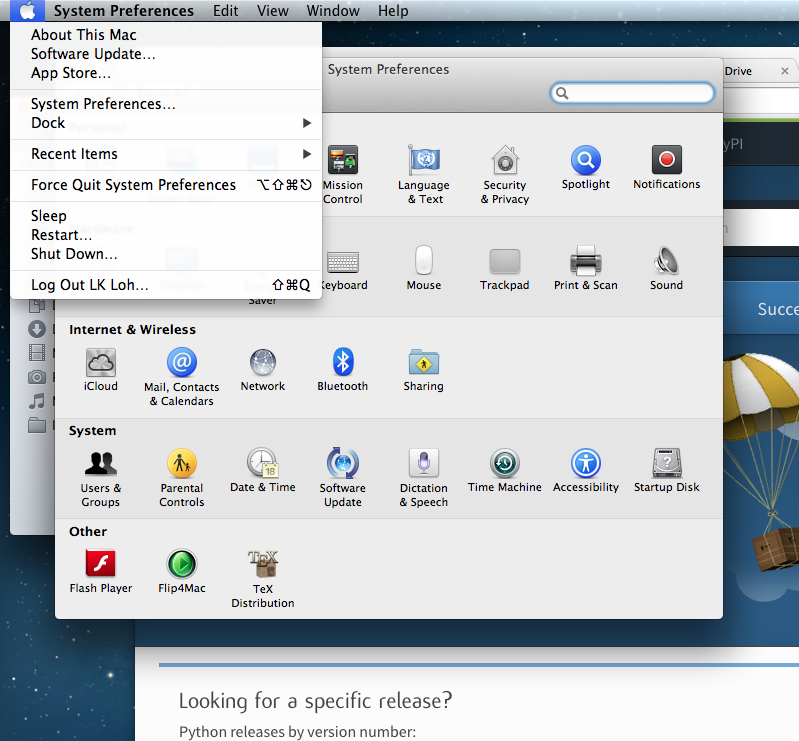
\includegraphics[width=0.5\textwidth]{images/system_preferences}
  \caption{Console}
  \label{fig:system_preferences}
\end{figure}

\begin{figure}[h!]
  \centering
  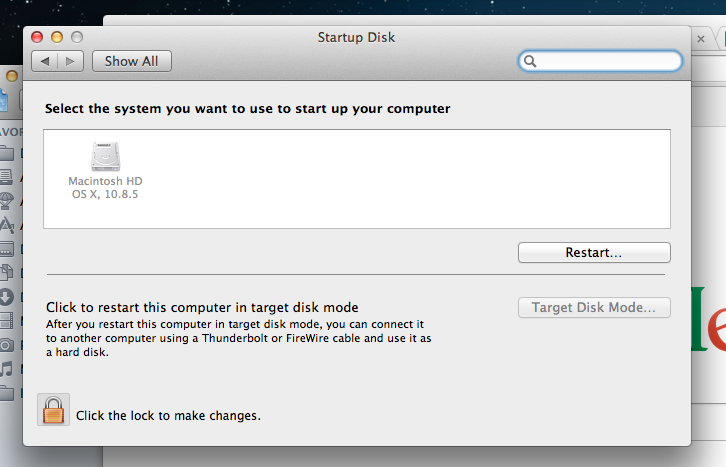
\includegraphics[width=0.5\textwidth]{images/startup_disk}
  \caption{Console}
  \label{fig:startup_disk}
\end{figure}

% -------------------------------------------------------------------------------------- %

\section{Installing Python}

\subsection{Getting Python}

Usually, Macs already have python installed by default. To check if you have python on your mac,
open up terminal, and do python in the terminal. If python is installed you should see some souch of console show up, as in Figure~\ref{fig:python_console}. If python is not installed, you should see an error message show up. 

\begin{figure}[h!]
  \centering
  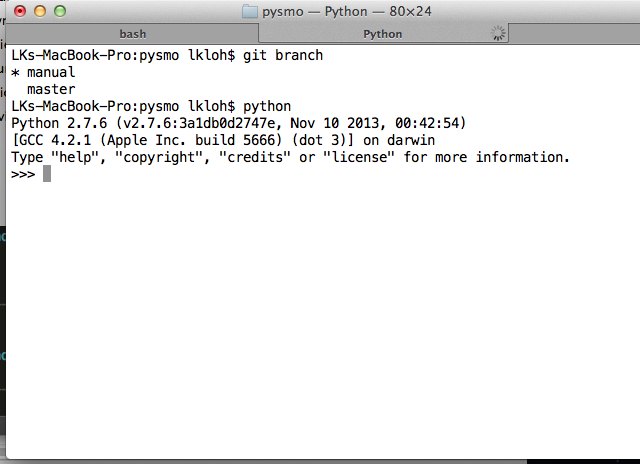
\includegraphics[width=0.5\textwidth]{images/python_console}
  \caption{Console}
  \label{fig:python_console}
\end{figure}

To get python, go to \url{https://www.python.org/}, and get the correct version for your operatin system. 

\begin{figure}[h!]
  \centering
  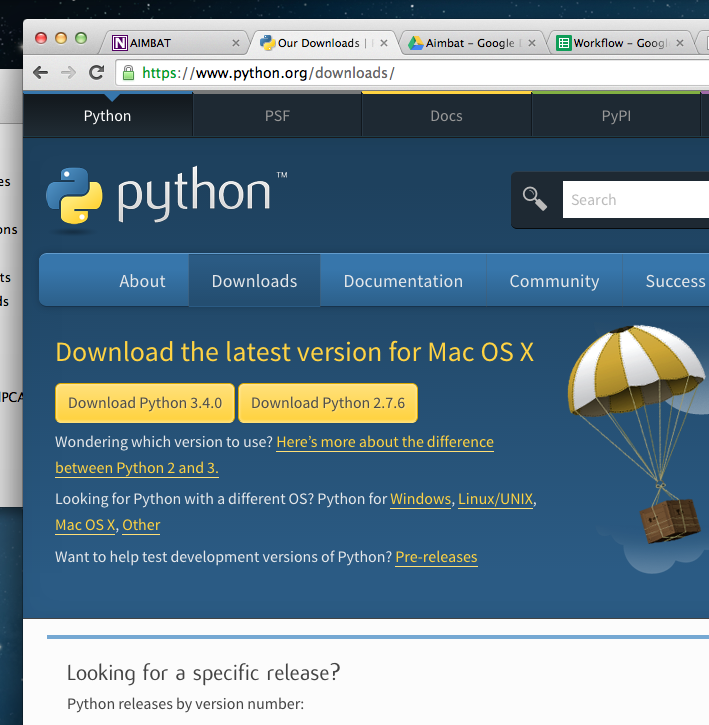
\includegraphics[width=0.5\textwidth]{images/python_version}
  \caption{Console}
  \label{fig:python_version}
\end{figure}



% -------------------------------------------------------------------------------------- %


\end{document}

% ---------------------------------------- END ---------------------------------------- %
